%%%% using 'arara' 4.0
% arara: xelatex: {synctex: yes, interaction: nonstopmode}
% arara: bibtex
% arara: xelatex: {synctex: yes, interaction: nonstopmode}
% arara: xelatex: {synctex: yes, interaction: nonstopmode}

% arara: indent: {overwrite: yes}

% arara: clean: { extensions: [aux, bcf, cod, blg, lof, lot, out, toc, log, xml, bak0 ] }

\documentclass[review]{elsarticle}

% Figures Links, mittig und rechts platzieren
\usepackage[export]{adjustbox}
\usepackage{caption}
\usepackage{subcaption}
\usepackage{amsmath}

% prevents that appendices are moved behind references
\usepackage{placeins}

\usepackage[nolist]{acronym}

\usepackage{longtable}
\usepackage{booktabs}
\usepackage{multirow}
\usepackage{float}

% enable linking to subsubsection
\setcounter{secnumdepth}{3}

% various symbols, e.g. \degree
\usepackage{gensymb}

\usepackage[hidelinks]{hyperref}

\usepackage{lineno}
\modulolinenumbers[5]

% set autoref abbr for appendix
\newcommand*{\Appendixautorefname}{appendix}

\journal{Journal "Remote Sensing of environment"}

% line breaks in table cells
\newcommand{\specialcell}[2][l]{%
  \begin{tabular}[#1]{@{}l@{}}#2\end{tabular}}

% tilde
\newcommand{\mytilde}{\raise.17ex\hbox{$\scriptstyle\mathtt{\sim}$}}

%% APA style
\bibliographystyle{model5-names}\biboptions{authoryear}

\begin{document}

\begin{frontmatter}

	\title{title}

	%% Group authors per affiliation:
	\author[FSU]{Patrick Schratz}
	\cortext[mycorrespondingauthor]{Corresponding author}
	\ead{patrick.schratz@uni-jena.de}

	\author[FSU]{Jannes Muenchow}
	\author[NEIKER]{Eugenia Iturritxa}
	%\author[TUDO]{Jakob Richter}
	\author[FSU]{Alexander Brenning}

	\address[FSU]{Department of Geography, GIScience group, Grietgasse 6, 07743, Jena, Germany}
	%\address[NEIKER]{NEIKER, Granja Modelo –Arkaute, Apdo. 46, 01080 Vitoria-Gasteiz, Arab, Spain}
	%\address[TUDO]{Department of Statistics, TU Dortmund University, Germany}

	\begin{abstract}

	\end{abstract}

	\begin{keyword}
		hyperspectral imagery \sep statistical learning \sep spatial cross-validation
	\end{keyword}

\end{frontmatter}

\linenumbers

% längste Abkürzung steht hier!!! in eckigen Klammern
\begin{acronym}[AUROC]

	% geringerer Zeilenabstand
	%\setlength{\itemsep}{-\parsep}
	\acro{ANN}{Artificial Neural Network}
	\acro{AUROC}{Area Under the Receiver Operating Characteristics Curve}
	\acro{BRT}{Boosted Regression Trees}
	\acro{CART}{Classification and Regression Trees}
	\acro{CV}{cross-validation}
	\acro{ENM}{Environmental Niche Modeling}
	\acro{FPR}{False Positive Rate}
	\acro{GAM}{Generalized Additive Model}
	\acro{GBM}{Gradient Boosting Machine}
	\acro{GLM}{Generalized Linear Model}
	\acro{ICGC}{Institut Cartografic i Geologic de Catalunya}
	\acro{IQR}{Interquartile Range}
	\acro{WKNN}{Weighted $k$-nearest neighbor}
	\acro{MARS}{Multivariate Adaptive Regression Splines}
	\acro{MEM}{Maximum Entropy Model}
	\acro{NRI}{Normalized Ratio Index}
	\acro{LOWESS}{Locally Weighted Scatter Plot Smoothing}
	\acro{PISR}{Potential Incoming Solar Radiation}
	\acro{RBF}{Radial Basis Function}
	\acro{RF}{Random Forest}
	\acro{SDM}{Species Distribution Modeling}
	\acro{SVM}{Support Vector Machines}
	\acro{TPR}{True Positive Rate}
\end{acronym}

\section{Introduction}
\label{sec:intro}

\section{Data and study area}

\subsection{Ground data}
% Describe Plots

The four \textit{Pinus radiata} plots Laukiz 1, Laukiz 2, Luiando and Oiartzun are located in the northern part of the Basque Country (\autoref{fig:study_area}).
Laukiz 1 has the most trees (n = 559) while Laukiz 2 has largest area size.
All plots besides Luiando are located nearby the coast.
The data was collected in September 2016.

% Show Map

\begin{figure} [t!]
	\begin{center}
		\makebox[\textwidth]{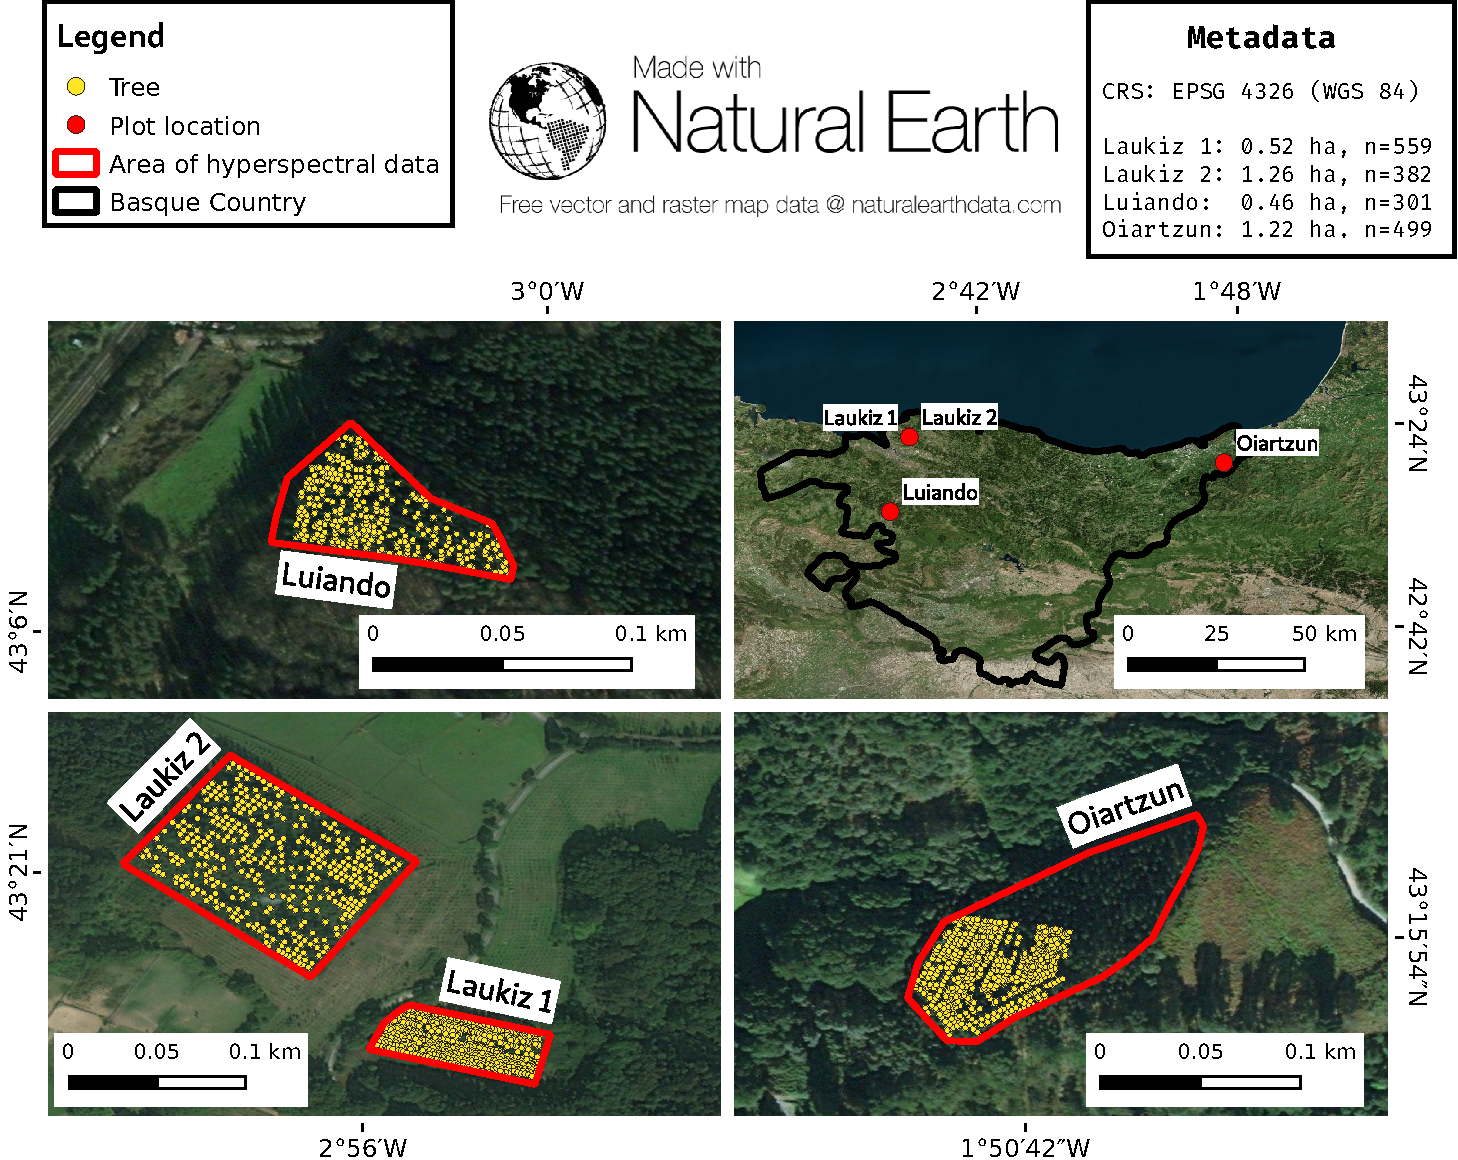
\includegraphics[width=\textwidth] {../03_figures/data/study_area_hyperspectral.pdf}}
		\caption{Information about the plot locations, the area of hyperspectral coverage and the number of trees per plot.}
		\label{fig:study_area}
	\end{center}
\end{figure}

% describe the hyperspectral data


\cite{Brenning2012}

% \begin{figure} [t!]
% 	\begin{center}
% 		\makebox[\textwidth]{\includegraphics[width=\textwidth] {../../04_figures/01_data/study_area.pdf}}
% 		\caption[Study area]{Spatial distribution of tree observations within the Basque Country, northern Spain, showing infection state by \textit{Diplodia sapinea}.}
% 		\label{fig: study_area}
% 	\end{center}
% \end{figure}

\subsection{Hyperspectral data}

The airborne hyperspectral data was acquired during two flight campaigns on September 28th and October 5th 2016, both around 12 am.
The images were taken by an AISAEAGLE-II sensor from the \ac{ICGC}.
All preprocessing steps (geometric, radiometric, atmospheric) have been conducted by \ac{ICGC}.

Additional information is provided in Table 1:

% parameter limits
\begin{table}[b!]
\centering
\caption[t]{Specifications of hyperspectral data.}
\begingroup\footnotesize
\begin{tabular}{ll}
	\\
	Characteristic         & Value                               \\
	\hline
	Geometric resolution   & 1 m                                 \\
	Radiometric resolution & 12 bit                              \\
	Spectral resolution    & 126 bands (404.08 nm - 996.31 nm)   \\
	Correction:            & Radiometric, geometric, atmospheric
\end{tabular}
\endgroup
\label{tab:hyperparameter_limits}
\end{table}



\section{Methods}

\subsection{Derivation of indices}

% link to PDF with veg indeces
All vegetation indices (90 total) suitable for the wavelength range of the hyperspectral data that are offered by the \texttt{hsdar} package have been calculated.
Additionally, all possible \ac{NRI} were calculated from the data using the formula:

\begin{equation}
	NRI_{i,j} = \frac{B_{i} - B_{j}}{B_{i} + B_{j}}
\end{equation}

\noindent
where $i$ and $j$ are the respective band numbers.

%To account for geometric offsets, we calculated every index five times using a buffer from 1 - 5 meter around the centroid of the respective tree.
To account for geometric offsets, we used a buffer of 2 meters around the centroid of the respective tree.
The mean value of all pixels touched by the buffer was assigned as the final value for each index.
Missing values were removed from the mean value calculation.
In total, 7875 \ac{NRI}s have been calculated ($\frac{125*126}{2}$).
Some indices returned \texttt{NA} values for some observations and were removed from the dataset, leaving a total of 7471 indices that were available for all plots without missing values.
Note that due to the mass of variables we cannot state which indices in detail have been removed.

\subsection{Penalized regression}

Penalized regression was used to account for the large amount of highly correlated predictor variables.
The aim was to find the indices that best explain defoliation within the plots.

Due to the amount of highly correlated predictors in the dataset, the independence assumption of the predictors is violated.
To compensate for that, penalized regression penalizes the coefficients.
This leads to a substantial decrease in variance and better predictive performance.
However, it also results in biased coefficients that cannot be used for statistical inference anymore.
The resulting coefficients can be seen as a measure of variable importance.
The penalization terms that have been used in this work are explained in the following sections.

\subsubsection{L1 Penalization}

\subsubsection{L2 Penalization}

\subsubsection{Elasticnet}

\subsection{Modeling}

The first step was to decide which penalization term works best for the given data.
A nested 10-fold spatial \ac{CV} was conducted on every single plot and for the merged dataset, we ran a plot-based \ac{CV} for both performance evaluation and hyperparameter tuning.
% show plot of spatial partitioning for both?
This means that three out of the 4 plots formed the training set while the test set consisted of the remaining plot.

Next, we applied the winning method (Ridge) again on the plots and the merged dataset to find the most important coefficients for every plot.
Hyperparameter tuning of

% Points to mention
% * All penalization methods are suited for different kinds of dataset structures
% * Find out which one works best on average and then use this method to create create models for prediction and variable importance

\section{Discussion}

\subsection{Index derivation}

The exact number of contributing pixels of an index cannot be determined as it depends on the location of the tree within the pixel grid.
If a tree is located at the border of a pixel, the same buffer (e.g. 3 m) will include more pixels than if the point is located at the center of a pixel.
Also, if a tree is located at the border of the image data, some directions of the buffer may not contain values.

\section*{References}

\bibliography{Biblio_hyperspectral}

\end{document}
